\documentclass[]{final_report}
\usepackage{graphicx}
\usepackage{hyperref}
\usepackage[final]{pdfpages}
\usepackage{booktabs}
\usepackage{multirow}
\usepackage{framed}
\usepackage{caption}
\usepackage{tikz}
\usetikzlibrary{timeline}
\usepackage{dirtree}

%%%%%%%%%%%%%%%%%%%%%%
%%% Input project details
\def\studentname{James King}
\def\reportyear{2018}
\def\projecttitle{Cooperative Strategies in Multi-Agent Systems}
\def\supervisorname{Kostas Stathis}
\def\degree{BSc (Hons) in Computer Science}
\def\fullOrHalfUnit{Full Unit} % indicate if you are doing the project as a Full Unit or Half Unit
\def\finalOrInterim{Final Report} % indicate if this document is your Final Report or Interim Report

\begin{document}

Tips:\begin{itemize}
	\item Communicate with Kostas
	\item Use figures!
	\item Ensure structure is flowing
	\item Use sources for everything
	\item Modularise in order to convert to paper
\end{itemize}
To Do:
\begin{itemize}
	\item Modularise in order to convert to paper
	\item Describe appendix
	\item Act on Interim Review Feedback
	\item Act on planning and timescale comments from interim report
	\item Act on contents of summary of completed work from interim report
	\item Change the Rationale to fit Final report
	\item Write a literature review or combine with Rationale and add to it?
	\item Write Contents and Knowledge
	\item Write critical analysis and discussion
	\item Write professional issues (get background reading and citations)
\end{itemize}
	
\maketitle

%%%%%%%%%%%%%%%%%%%%%%
%%% Declaration

\chapter*{Declaration}

This report has been prepared on the basis of my own work. Where other published and unpublished source materials have been used, these have been acknowledged.

\vskip3em

Word Count:

\vskip3em

Student Name: \studentname

\vskip3em

Date of Submission: \today

\vskip3em

Signature: \\

\includegraphics[scale=0.05]{Signature.png}

\newpage

%%%%%%%%%%%%%%%%%%%%%%
%%% Table of Contents
\tableofcontents\pdfbookmark[0]{Table of Contents}{toc}\newpage

%%%%%%%%%%%%%%%%%%%%%%
%%% Your Abstract here

\begin{abstract}
\end{abstract}
\newpage

\chapter{Introduction}
\section{Motivation}
Problem statement and associated objectives.\\
Give a rationale.
\section{Aims and Objectives}

\section{Contribution}

\section{Structure}


\chapter{Background}
\section{Introduction}
Include background reading\\
Critical lit review.\\
Comprehensive knowledge.\\

\section{Literature Review}

\section{Technique 1}
Description, limitations, our technique\\
Examples:
\begin{itemize}
	\item Evolcoop Axerlrod, Axelrod.py
	\item Arithmetics of mutual help
	\item Pheklps, game theoretic analysis
	\item 5 rules coop
	\item spatial and graphs
	\item Evol indirect image, Nowak and Sigmund
	\item multilevel nowak
	\item Genetic drift as an issue
	\item gossip alternative
	\item rational cooperation in finite iterated prisoners
	\item prisoners and their dilemma
	\item evol dir indir
	\item evol of coop through indir rec
	\item kin hamilton
	\item image vs standing
	\item notions of reputation in mas
\end{itemize}

\section{Technique 2}
Description, limitations, our technique

\section{Technique n}
Description, limitations, our technique

\section{Summary}
Summarise limitations and the tecniques we are using to combat this

\chapter{Framework}
 Excellent understanding and insight. Concep
 tual framework underpins study. Comprehensive
 expert account of topic. Well thought through Software Engineering content.

\section{Theoretical}
Relate to background.

\section{Implementation}
Relate to agents systems.
\subsection{Agents Service}
\subsection{Environment}
\subsection{Web Application and Interface}
\subsection{Conclusion}

\section{Technical Preparation}
Learning flask etc.

\section{Design}

\subsection{Agents Service}
\subsection{Environment}
\subsection{Web Application and Interface}

\section{Development}

\subsection{Agents Service}
\subsection{Environment}
\subsection{Web Application and Interface}

\section{Testing}

\subsection{Agents Service Testing}
\subsection{Environment Testing}
\subsection{Web Application Testing}

\section{Software Engineering}

\section{Documentation}
Software documentation, user guide.

\section{Experiment Evaluation}

\subsection{Experiment 1}
Variable setting, controls etc.\\
Evaluation

\subsection{Experiment 2}

\subsection{Experiment n}

\subsection{Discussion}
Evaluation and discussion on the experiments\\
Successful?\\
Opportunity for extra work?\\
Focus on experiments

\chapter{Critical Analysis and Discussion}
Project achievements\\
Reflection on project process (difficulties, success, failure)\\
Successful?\\
Future enhancements\\
Focus on project\\
Compare to deliverables at beginning.

\chapter{Conclusions}
Opportunity for extra work?

%%%% ADD YOUR BIBLIOGRAPHY HERE
\newpage
\bibliography{../../refs.bib}{}
\bibliographystyle{plain}
\addcontentsline{toc}{chapter}{Bibliography}
\footnote{A lot of my background theory work has been completed in my earlier reports so many of the references appear in those reports (see appendix)}
\label{endpage}

\chapter{Professional Issues}
Replacement of people in jobs?\\
AI issues and risks?\\
Relate to project

\chapter{Appendix}
\label{appendix}
Describe the contents of my appendix.

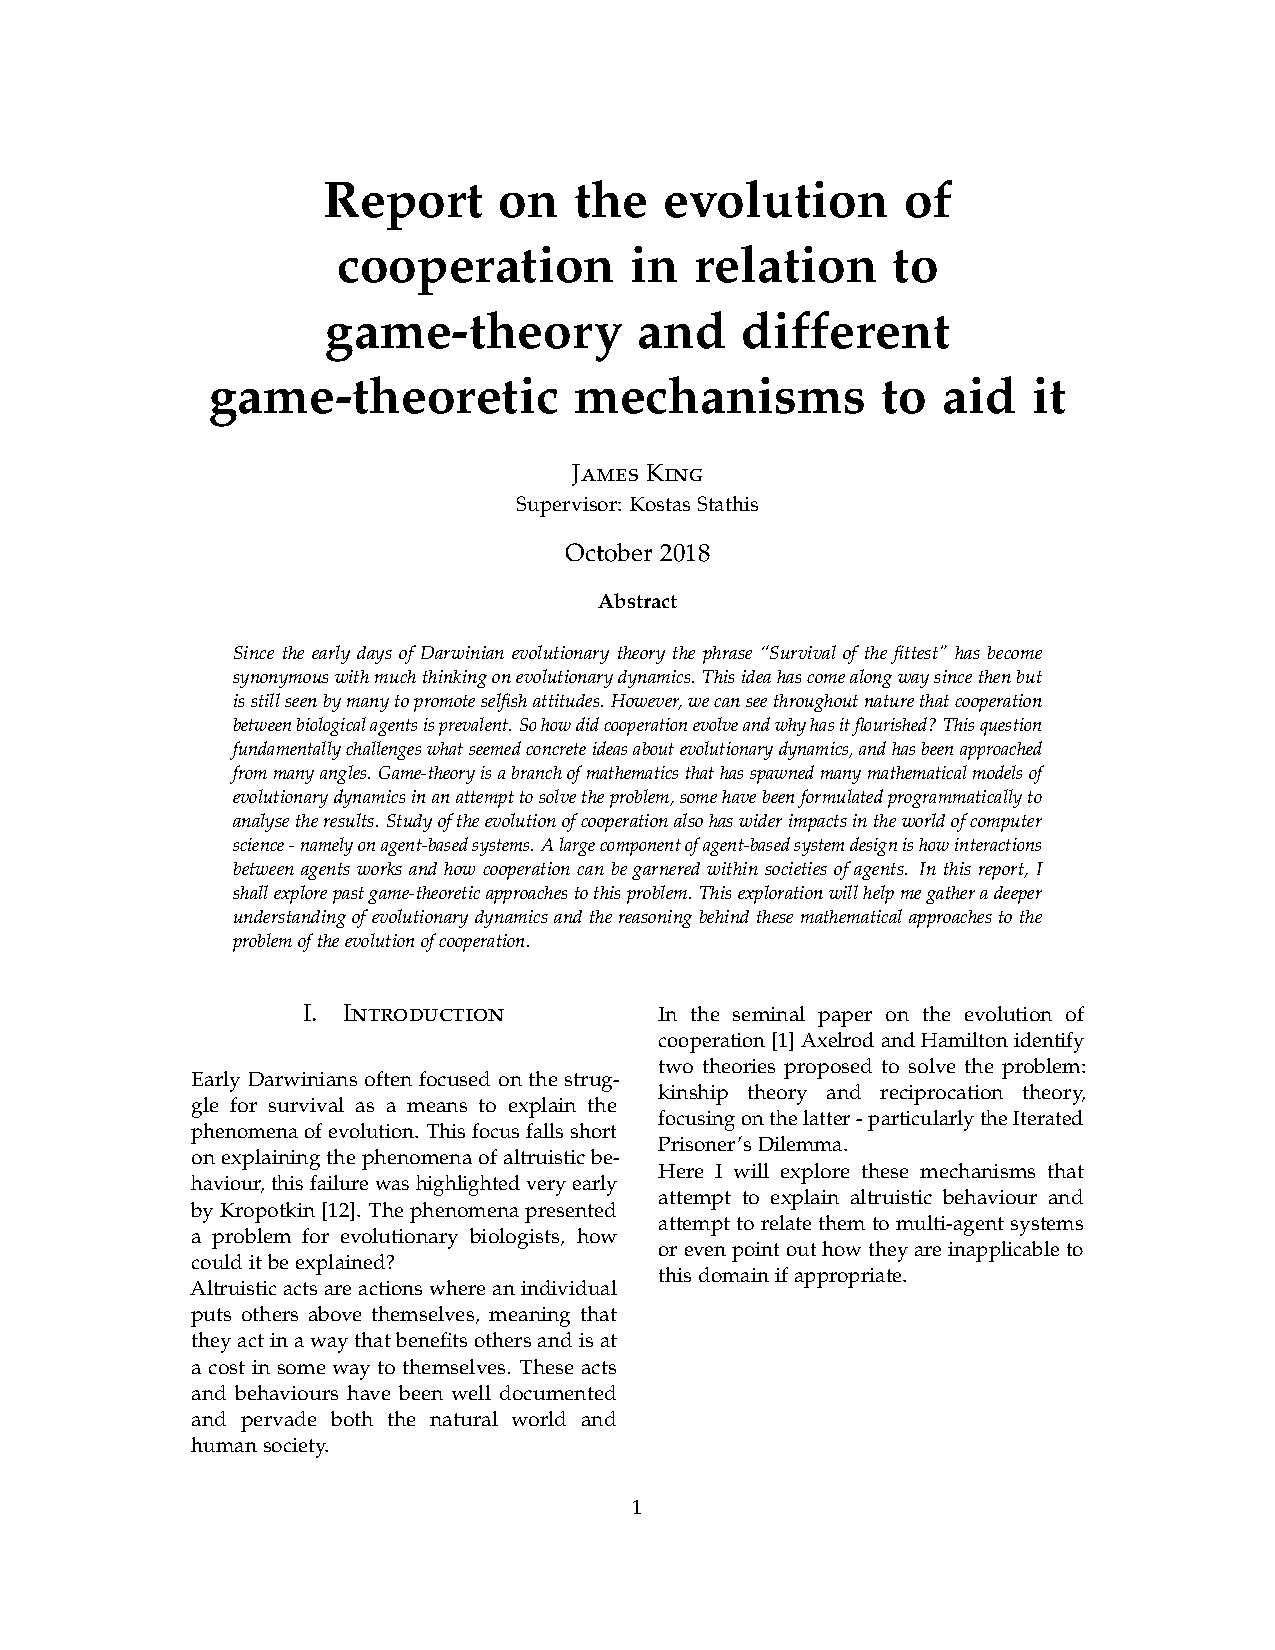
\includepdf[pages=-]{../../EvolCoop/EvolCoopReport.pdf}

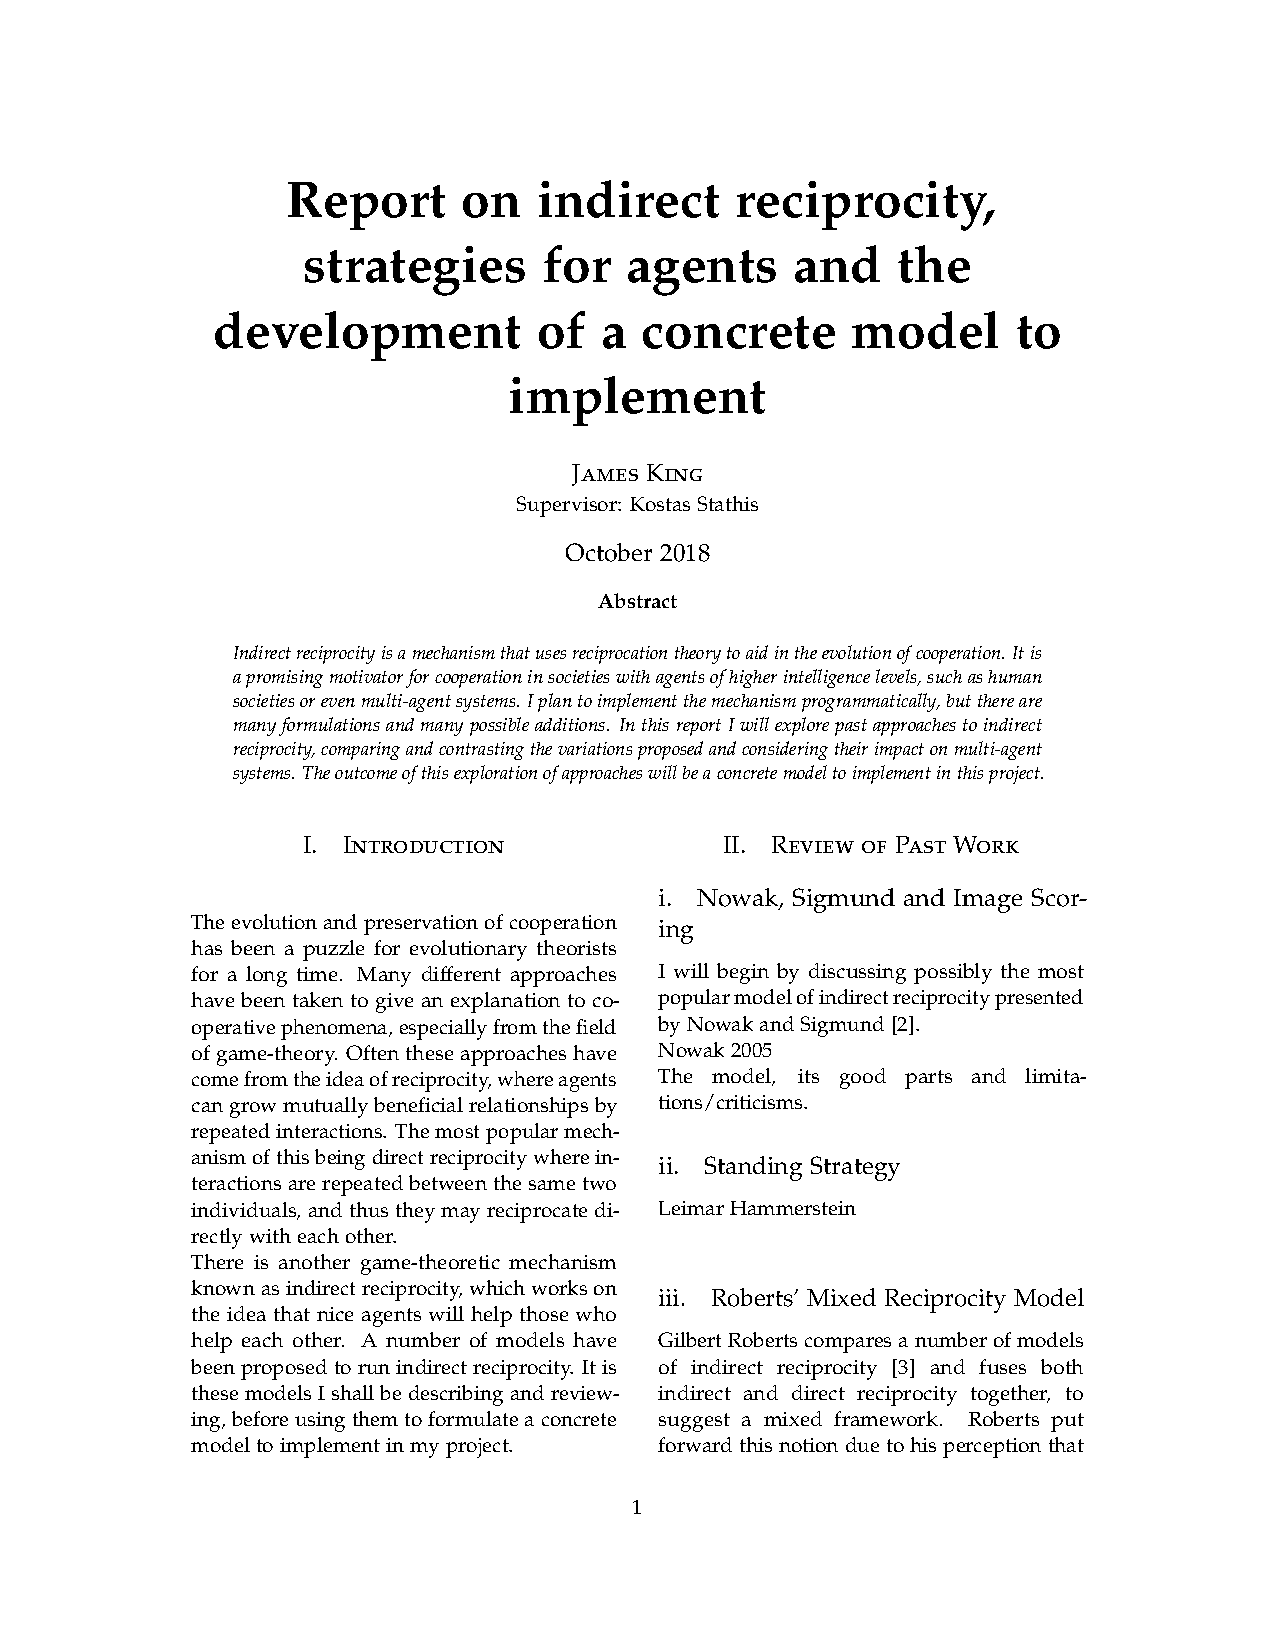
\includepdf[pages=-]{../../IndirRec/IndirRec.pdf}

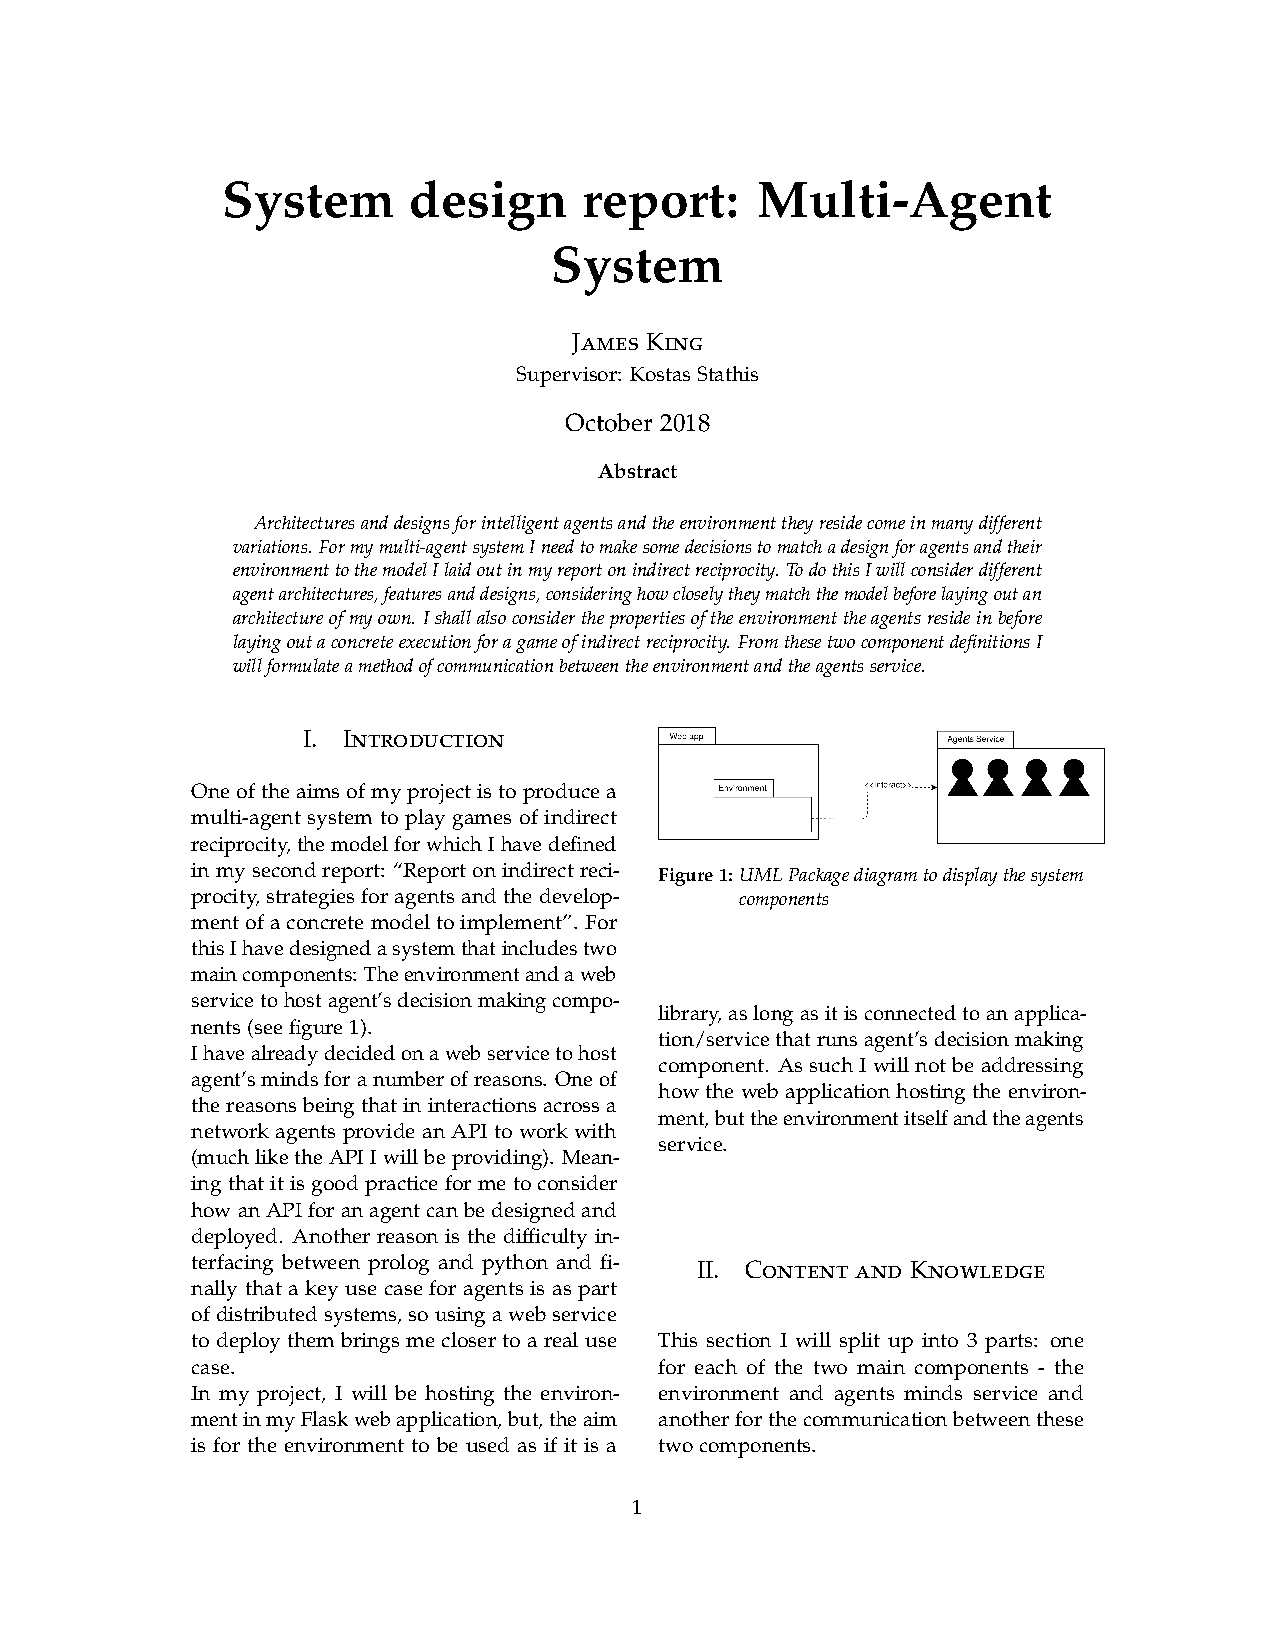
\includepdf[pages=-]{../../SysDesign/SysDesign.pdf}

\begin{figure}
	
\includepdf[pages=-,link=true,linkname=web_app_testing]{../../TestingStrategy/TestingStrategy.pdf}
	\caption{\label{appendix:web_app_testing}}
	
\end{figure}


\end{document}

\end{article}
